\newpage % Rozdziały zaczynamy od nowej strony.
 

\section{Użyte metody}
W tym rozdziale opiszę użyte przez siebie metody prowadzące, od zbioru kodów źródłowych programów, do działającego modelu 
przewidującej kolejny token w programie. \\\\\\ 

\subsection{Badane modele}
Rekurencyjne sieci neuronowe należą do rodziny sieci służących do przetwarzania sekwencji danych o określonej długości. Jak pokazali w swojej publikacji 
autorzy \cite{lstmvsgru}, sieć LSTM osiąga znacznie lepsze wyniki od sieci rekurencyjnych Hopfielda \cite{hopfield} oraz minimalnie lepsze wyniki 
od sieci GRU, kosztem dłuższego czasu treningu. Z tego względu w swoich badaniach skupiam się głównie na warstwie LSTM oraz w mniejszej mierze na warstwie GRU, 
która również wyprzedza sieć Hopfielda pod względem skuteczności. 

Wszystkie eksperymenty badające wpływ hiperparametrów przeprowadzę na sieci LSTM, oraz najlepszą ich kombinację 
zbadam przy wykorzystaniu warstwy GRU w celu porównania ich skuteczności w zadaniu przewidywaniu kodu. Na koniec zbadam również zachowanie wyznaczonego modelu 
dla różnych rozmiarów słownika. 

Jak pokazał w swojej pracy Yoon Kim \cite{kim} połączenie warstwy rekurencyjnej z warstwą zanurzeń poprzez warstwę splotową może mieć pozytywny wpływ na skuteczność 
modelu. Jednak badanie to wykonywał jedynie w zadaniu modelowania języka naturalnego oraz dla modeli opartych na pojedyńczych znakach. Jednym z wykonanych przeze mnie 
eksperymentów będzie zastosowanie tej techniki w moim zadaniu, oraz oceny skuteczności tego podejścia dla modeli opartych na tokenach. 

Ogólny badany przeze mnie model uczenia głębokiego został przedstawiony na rysunku \ref{fig:architektura}. Składa się on z sieci zanurzeń, opcjonalnej warstwy CNN, 1 lub 2 
warstw rekurencyjnych LSTM, oraz warstwy klasyfikującej.

Na architekturę całej wtyczki składa się wybrany przeze mnie model uczenia głębokiego połączony z 2 modelami typu n-gram. Zasada działania tej kombinacji 
została opisana w rozdziale \ref{oov}. 

\begin{figure}[!h]
	% Znacznik \caption oprócz podpisu służy również do wygenerowania numeru obrazka;
	\caption{Ogólny badany model. Opcjonalne warstwy zaznaczone linią przerywaną}
	% dlatego zawsze pamiętaj używać najpierw \caption, a potem \label
    \label{fig:architektura}
    % Zamiast width można też użyć height, etc. 
    \centering 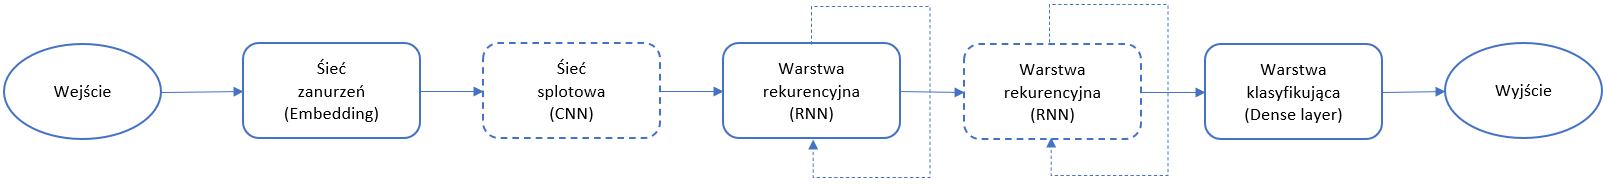
\includegraphics[width=160mm, height=25mm]{architektura.png}
\end{figure}


\begin{table}[ht]
    \centering
    \resizebox{\textwidth}{!}{\begin{tabular}{ccccc}
            \hline
            \multicolumn{1}{|c|}{Długość sekwencji}   & \multicolumn{1}{c|}{Warstwa CNN}          & \multicolumn{1}{c|}{Liczba warstw LSTM} & \multicolumn{1}{c|}{Liczba neuronów w warstwie} & \multicolumn{1}{c|}{Liczba wszystkich wag} \\ \hline
            \multicolumn{1}{|c|}{1}                   & \multicolumn{1}{c|}{nie}                  & \multicolumn{1}{c|}{1}                  & \multicolumn{1}{c|}{512}                        & \multicolumn{1}{r|}{12,016,705}                         \\ \hline
            \multicolumn{1}{|c|}{\multirow{5}{*}{5}}  & \multicolumn{1}{c|}{\multirow{4}{*}{nie}} & \multicolumn{1}{c|}{\multirow{3}{*}{1}} & \multicolumn{1}{c|}{128}                        & \multicolumn{1}{r|}{3,302,593}                         \\ \cline{4-5} 
            \multicolumn{1}{|c|}{}                    & \multicolumn{1}{c|}{}                     & \multicolumn{1}{c|}{}                   & \multicolumn{1}{c|}{256}                        & \multicolumn{1}{r|}{6,076,225}                         \\ \cline{4-5} 
            \multicolumn{1}{|c|}{}                    & \multicolumn{1}{c|}{}                     & \multicolumn{1}{c|}{}                   & \multicolumn{1}{c|}{512}                        & \multicolumn{1}{r|}{12,016,705}                         \\ \cline{3-5} 
            \multicolumn{1}{|c|}{}                    & \multicolumn{1}{c|}{}                     & \multicolumn{1}{c|}{2}                  & \multicolumn{1}{c|}{128}                        & \multicolumn{1}{r|}{3,434,177}                         \\ \cline{2-5} 
            \multicolumn{1}{|c|}{}                    & \multicolumn{1}{c|}{tak}                  & \multicolumn{1}{c|}{1}                  & \multicolumn{1}{c|}{128}                        & \multicolumn{1}{r|}{3,303,649}                         \\ \hline
            \multicolumn{1}{|c|}{\multirow{5}{*}{10}} & \multicolumn{1}{c|}{\multirow{4}{*}{nie}} & \multicolumn{1}{c|}{\multirow{2}{*}{1}} & \multicolumn{1}{c|}{128}                        & \multicolumn{1}{r|}{3,302,593}                         \\ \cline{4-5} 
            \multicolumn{1}{|c|}{}                    & \multicolumn{1}{c|}{}                     & \multicolumn{1}{c|}{}                   & \multicolumn{1}{c|}{512}                        & \multicolumn{1}{r|}{12,016,705}                         \\ \cline{3-5} 
            \multicolumn{1}{|c|}{}                    & \multicolumn{1}{c|}{}                     & \multicolumn{1}{c|}{2}                  & \multicolumn{1}{c|}{128}                        & \multicolumn{1}{r|}{3,434,177}                         \\ \cline{3-5} 
            \multicolumn{1}{|c|}{}                    & \multicolumn{1}{c|}{}                     & \multicolumn{1}{c|}{2}                  & \multicolumn{1}{c|}{512}                        & \multicolumn{1}{r|}{14,115,905}                         \\ \cline{2-5} 
            \multicolumn{1}{|c|}{}                    & \multicolumn{1}{c|}{tak}                  & \multicolumn{1}{c|}{1}                  & \multicolumn{1}{c|}{128}                        & \multicolumn{1}{r|}{3,303,649}                         \\ \hline
            \multicolumn{1}{|c|}{\multirow{2}{*}{15}} & \multicolumn{1}{c|}{\multirow{2}{*}{nie}} & \multicolumn{1}{c|}{\multirow{2}{*}{1}} & \multicolumn{1}{c|}{128}                        & \multicolumn{1}{r|}{3,302,593}                         \\ \cline{4-5} 
            \multicolumn{1}{|c|}{}                    & \multicolumn{1}{c|}{}                     & \multicolumn{1}{c|}{}                   & \multicolumn{1}{c|}{512}                        & \multicolumn{1}{r|}{12,016,705}                         \\ \hline
            \end{tabular}}
    \caption{Zestawienie wykonywanych eksperymentów} 
    \label{eksperymenty}
\end{table} 
Zdecydowałem, że nie ma potrzeby testowania wszystkich możliwych kombinacji parametrów w tabeli, ponieważ zajęło by to bardzo dużo czasu, oraz już na podstawie prac 
\cite{hellendoorn, pythia} możemy łatwo stwierdzić, że część kombinacji nie osiągnie konkurencyjnych wyników przy pozostałych, na przykład pojedyńcza warstwa LSTM, o 
128 komórkach i długości okna równej \begin{math}1\end{math} jest zdecydowanie za prostym modelem aby przechwycić wszystkie zależności między danymi. Przeprowadzane 
przeze mnie eksperymenty przedstawione są w tabeli \ref{eksperymenty}. 

\subsection{Hiperparametry}
Badając różne w możliwości układów warstw należy rozważyć kilka szczególnych kwestii dotyczących hiperparametrów testowanych przeze mnie modeli. 
Poszczególnie zbadam 
\begin{itemize}
    \item dla jakiej długości sekwencji wejściowej model osiągnie najlepsze wyniki,
    \item jak rozmiar słownika wpływa na skuteczność modelu, 
    \item jaka liczba warstw rekurencyjnych osiągnie najlepsze wyniki,
    \item dla jakiej liczby neuronów w warstwie model osiągnie najlepsze wyniki, 
    \item jaki wpływ ma warstwa CNN, 
    \item który rodzaj warstw rekurencyjnych osiągnie najlepsze wyniki.
\end{itemize}
\subsection{Projektowanie wtyczki}
\begin{description}
\item[Wstępne przetwarzanie danych]
\hfill \\
Przed dostarczeniem danych do modelu zostają one odpowiednio przetworzone. Operacja ta polega na usunięciu wszystkich wykomentowanych linii kodu 
w celu zapobięgnięcia uczenia modelu na słowach nie będących kodem. Następnie usuwane są wszystkie puste linie gdyż nie niosą one żadnej informacji o 
kolejnych tokenach. Ostatnim krokiem jest usunięcie wcięć w kodzie, gdyż wynikają one ze struktury programów w języku python, przez co próba przewidywania  
ich przy pomocy uczenia maszynowego nie ma sensu. \\

\item[Modelowanie tokenów]
\hfill \\
Jak pokazują w swojej publikacji autorzy \cite{character-level} mimo tego, że modele budujące kolejne słowa poprzez 
przewidywanie pojedyńczego znaku (character-level model) radzą sobie dobrze z modelowaniem języka naturalnego, oraz rozwiązują problem rozmiaru słownika, 
działają znacznie gorzej z językami programowania. Wniosek ten również potwierdza w swojej pracy autor \cite{erik} porównując model przewidujący 
znaki z modelem przewidującym tokeny. Z tego powodu realizuję tylko modele oparte na tokenach (token-level model). 

Pierwszym krokiem jest zbudowanie słownika tokenów, które mogą pojawić się w kodzie. Buduję go poprzez przetworzenie wszystkich kodów źródłowych obu zbiorów treningowego oraz 
walidacyjnego modułem tokenize \cite{tokenize} wbudowanym w język Python. Moduł ten przyjmuje na wejściu kod źródłowy programu następnie zwraca listę kolejnych tokenów (nazw zmiennych, 
znaków specjalnych, słów kluczowych). Upewnia się on również czy kod jest poprawnie napisany, na przykład czy wszystkie nawiasy lub apostrofy zostały zamknięte. Pliki zawierające błędy w 
kodzie zostają pominięte. 
Znaki nowej lini również traktuję jako token, jednak nie uwzględniam wcięć w kodzie ze względu na to, że większość środowisk programistycznych stawia je 
automatycznie. Na przykład z kodu źródłowego: 
\begin{addmargin}[10mm]{0mm}
    \begin{lstlisting}[
        language=Python,
        numbers=left,
        firstnumber=1,
        caption={Przykładowy program Python},
        aboveskip=10pt
    ]
    for x in range(2, 10): 
        print("hello world")
    \end{lstlisting}
    \end{addmargin}
otrzymamy listę \textbf{ [for, x, in, range, (, 2, 10, ), :, \textbackslash n, print, (, "hello world", )]}.
Następnie sortuje wszystkie wygenerowane tokeny według częstości występowania oraz wybieram top-n tokenów jako słownik i każdemu z nich przypisuję unikalną liczbę naturalną. 
Utworzony w ten sposób słownik nie jest kompletny ponieważ nie obejmuje on wszystkich możliwych nazw występujących w kodzie. Takiego rodzaju tokeny
zostają zastąpione sztucznym tokenem '<UNKNOWN>'. W głównej mierze są to unikalne nazwy zmiennych oraz ciągi znaków. Zastępowanie tokenu '<UNKNOWN>' prawdziwym tokenem omawiam w 
rozdziale \ref{oov}\\

\item[Wybór podzbioru danych]
\hfill \\ 
Jak już wspomniałem w sekcji \ref{sec:dataset-background} dotyczącej zbioru danych, trening odbywa sie na podzbiorze wszystkich zgromadzonych danych. W tym celu wybrałem 9 najpopularniejszych, 
zewnętrznych bibliotek języka Python, stosowanych w zróżnicowanych dziedzinach rozwoju oprogramowania. Poniżej zamieszczam listę wybranych bibliotek, wraz z krótkim opisem:
\begin{itemize}
    \item Django - rozwój aplikacji sieciowych,
    \item Numpy - wykonywanie obliczeń matematycznych wysokiego poziomu,
    \item Requests - wysyłanie zapytań http, 
    \item Flask - rozwój aplikacji sieciowych,
    \item TensorFlow - Głębokie uczenie maszynowe,
    \item Keras - Wysokopoziomowe uczenie maszynowe,
    \item PyTorch - Głębokie uczenie maszynowe, 
    \item Pandas - Zarządzanie dużymi zbiorami danych, 
    \item PyQt - Tworzenie interfejsów użytkownika.
\end{itemize} 
Aby upewnić się, że wybrany przeze mnie zbiór danych poprawnie oddaje rzeczywistość porównałem liczbę plików źródłowych zwierających konkretną bibliotekę ze zbioru, z odpowiadającą 
liczbą wszystkich plików źródłowych na platformie GitHub \cite{github}. Stosunek tych dwóch liczb został przedstawiony w kolumnie 'Stosunek'. Zestawienie to znajduje się w tabeli \ref{tab:dataset-compare} 
\begin{table}[!h] \centering
    % Znacznik \caption oprócz podpisu służy również do wygenerowania numeru tabeli;
    \caption{Zestawienie zbioru danych z platformą GitHub}
    % dlatego zawsze pamiętaj używać najpierw \caption, a potem \label.
    \label{tab:dataset-compare}
    
    \begin{tabular} {| c | c | r | r |} \hline
        Biblioteka & Liczba plików GitHub & Liczba plików w zbiorze danych & Stosunek\\\hline\hline
        Django & 187000000 & 26732 & 0.014\% \\\hline
        Numpy & 55000000 & 9058 & 0.016\% \\ \hline
        Requests & 42000000 & 6339 & 0.015\%\\ \hline
        Pandas & 19000000 & 1328 & 0.007\%\\ \hline
        Flask & 17000000 & 3230 & 0.019\% \\ \hline
        TensorFlow & 10000000 & 96 & 0.001\%\\ \hline
        Keras & 3000000& 72 & 0.002\%\\ \hline
        PyQt & 1000000 & 132 & 0.013\%\\ \hline
        PyTorch & 1000000 & 0 & 0\%\\ \hline
    \end{tabular}
\end{table}

Jak możemy zaobserwować stosunek liczby plików jest dosyć zbliżony dla większości wybranych bibliotek wynosi około 0.015\%. Wyjątkami są 
biblioteki uczenia maszynowego. Może to wynikać z tego, że dane pochodzą z 2018 roku. Jest to czas, w którym istniały początkowe wersje tych bibliotek oraz dopiero
zaczynały zyskiwać na popularności. Od tego czasu również biblioteka Keras została scalona z biblioteką TensorFlow co znacznie wpłynęło na jej popularność w dzisiejszych czasach. 

Uznaję, że dane w wystarczająco dobrym stopniu oddają częstotliwość zastosowania bibliotek. Końcowy podzbiór stworzyłem poprzez wybranie 1\% plików źródłowych z każdej biblioteki. 
Końcowe zestawienie znajduje się w tabeli \ref{tab:dataset-compare-github}

\begin{table}[!h] \centering
    % Znacznik \caption oprócz podpisu służy również do wygenerowania numeru tabeli;
    \caption{Zestawienie zbioru i podzbioru danych}
    % dlatego zawsze pamiętaj używać najpierw \caption, a potem \label.
    \label{tab:dataset-compare-github}
    
    \begin{tabular} {| c | c | r | r |} \hline
         & Cały zbiór danych & Podzbiór treningowy & Podzbiór walidacyjny \\\hline\hline
        Pliki & 150000 & 9103 & 4504 \\\hline
        Tokeny & 114641650 & 9118453 & 4482600 \\ \hline
    \end{tabular}
\end{table}
Rozmiar wykorzystanego zbioru danych różni się do zbioru użytego w publikacji \cite{hellendoorn} w którym użyto 16 milionów tokenów do treningu, oraz 
5 milionów tokenów w celach walidacji. Na różnicę tą zdecydowałem się ze względu na ograniczenia sprzętowe różniące oba projekty. \\


\item[Trening]
\hfill\\ 
Zadanie polega na przewidzeniu kolejnego tokenu na podstawie zadanej sekwencji tokenów. Długość sekwencji jest stała oraz wyrażona poprzez wielkość okna będącą jednym z badanych hiperparametrów. 
Dla każdego z tokenów model wylicza jego wektor zanurzenia, wykonuje jeden krok w sieci rekurencyjnej po czym stosuje warstwę klasyfikującą 
(Dense layer) w celu wygenerowania logitów wyrażających logistyczne-prawdopodobieństwo kolejnego tokenu. Zatem dla zadanego okna tokenów długości \begin{math}W\end{math}:
\begin{math}[t_1, t_2, ... t_W]\end{math} obliczam wynik dla każdego możliwego wyjścia \begin{math}j, s_j\end{math} jako funkcję z wektorów tokenów \begin{math}v_{t_i}\end{math}
z tokenów z okna.\\
\centerline{\begin{math}g = [g_1, g_2, ..., g_W]\end{math}}
\centerline{\begin{math}[g_1, g_2, ..., g_W] = RNN([v_{t_1}, v_{t_2}, ..., v_{t_W}])\end{math}}
\centerline{\begin{math}s_j=p_{j}^{T}[g]\end{math}}\\\\
Minimalizowana funkcja strat jest entropią krzyżową pomiędzy prawdopodobieństwami \begin{math}softmax\end{math} dla każdego możliwego wyjścia 
a wykonaną predykcją.Funkcja wyrażoną wzorem: \\\\
\centerline{\begin{math}L = -log(\frac{exp(s_{t_o})}{\sum_{j}exp(s_{t_j})})\end{math}}\\\\
gdzie \begin{math}t_o\end{math} jest zaobserwowanym tokenem wyjściowym a \begin{math}g_i\end{math} wyjściem \begin{math}i-tej\end{math} komórki
którejś z badanych sieci rekurencyjnych. 

Wagi sieci aktualizowane są po przetworzeniu porcji danych (mini-batch), której rozmiar jest stały. Przy treningach sieci rekurencyjnych rozmiar
ten jest jedną z wartości kluczowych dla dobrej wydajności sieci. W moich eksperymentach wynosi on 128. Jest to kompromis pomiędzy rozsądnym 
czasem treningu oraz jakością wyjściowych sugestii. Jest to również najczęściej wybierana wartość w przytoczonych przeze mnie publikacjach.

Każda testowana architektura trenowana jest przez 25 epok. Wartość tą wybrałem na podstawie własnych eksperymentów wstępnych, z których wynika, że 
powyżej tej liczby model nie osiągał już lepszych rezultatów. Zbyt długi trening może również doprowadzić to przetrenowania modelu, czego 
należy unikać. 
\end{description}
\subsection{Ewaluacja}
\label{evaluation}
Jako, że badane przeze mnie modele tworzone są z myślą użycia ich w postaci wtyczki do środowiska programistycznego nie ma sensu ocenianie ich na podstawie pierwszej, najlepszej predykcji. 
Zamiast tego użyję dwóch następujących metryk: 

\begin{description}
    \item[Ewaluacja bez uwzględnienia kolejności] 
    \hfill \\ Jeśli poszukiwane słowo znajduje się w pierwszych \begin{math}n\end{math} najlepszych predykcjach, bez znaczenia na którym miejscu uważam sugestię za poprawną. Metrykę tą zastosowano przy ocenianiu systemów
    Pythia \cite{pythia} dla której \begin{math}n = 5\end{math} oraz w pracy \cite{contextual_code_completion} gdzie \begin{math}n = 3\end{math}. Zastosowanie jej pozwoli na porównanie 
    wyników z tymi publikacjami. Miara ta jest dalej nazywana "Top n"\\
    \item[Ewaluacja z uwzględnieniem kolejności] 
    \hfill \\ Jednym z przytoczonym problemów we wstępie \ref{sec:intro} jest to, że wiele wtyczek nie uwzględnia kolejności sugestii oraz proponuje je na przykład posortowane leksykograficznie. Proponowane przeze mnie rozwiązanie 
    sortuje predykcje na podstawie prawdopodobieństwa ich wystąpienia. Należy uwzględnić tą kolejność w metryce. Ocena obliczana jest poprzez podzielenie prawdopodobieństwa poprawnej predykcji przez 
    jego indeks w zbiorze zebranych predykcji. Dla przykładu powiedzmy, że model proponujący 10 sugestii zostaje użyty do wykonania 4 predykcji. Pierwsza wystąpi na 1. miejscu, druga na 3. miejscu, trzecia nie zmieści w w 10 najlepszych, 
    a czwarta na 8. miejscu. W takim przypadku ocena modelu będzie wynosić \begin{math}(\frac{1}{1}+ \frac{1}{3}+ 0 +\frac{1}{8})/4 = 0.36\end{math}. W ten sposób wyższe predykcje oceniane są zdecydowanie lepiej.
    Przy ocenie użyję 10 najlepszych sugestii.  Metryki tej używa Erik van Scharrenburg \cite{erik} w swojej pracy. Zastosowanie jej pozwoli na porównanie wyników. Miara ta jest dalej 
    nazywana "Top n z kolejnością" \\

  \end{description}


\subsection{Szczegóły implementacji}
\label{oov}
\begin{description}
\item[Problem słów poza słownikiem]
\hfill \\
Największym wyzwaniem przy modelowaniu języka programowanie jest rozwiązanie problemu słów poza słownikiem opisanego w podrozdziale \ref{zastosowania}. 
Jednym z podejść zastosowanym przez autorów \cite{contextual_code_completion} jest zastępowanie tokenów nie występujących w słowniku 
specjalnymi tokenami pozycyjnymi. Tego typu tokenowi, który powtarza się więcej niż raz w sekwencji, zostaje przypisany indeks jego wystąpienia 
odpowiadający jego pierwszemu wystąpieniu. W przypadku gdy przewidziany token nie mieści się w słowniku ale pojawił się wcześniej w 
sekwencji zostaje zastąpiony wcześniej podaną nazwą. Rozwiązanie to sprawdza się bardzo dobrze dla zmiennych o tej samej nazwie, znajdujących 
sie blisko siebie, na przykład w pętli \begin{math}for\end{math} języka \begin{math}C++\end{math}: 
\begin{addmargin}[10mm]{0mm}
    \begin{lstlisting}[
        language=C++,
        numbers=left,
        firstnumber=1,
        caption={Przeparsowana pętla for},
        aboveskip=10pt
    ]
    for (int POS_TOKEN_01=0; POS_TOKEN_01<10; POS_TOKEN_01++)
    \end{lstlisting}
    \end{addmargin}
Metoda ta jednak ogranicza się do długości badanej sekwencji, która jest bardzo krótka względem przeciętnej długości kodów programów.


Inną metodą jest zastosowanie warstwy splotowej zamiast warstwy zanurzeń zaproponowaną przez Yoon Kim \cite{kim}. Metoda ta osiąga skuteczność 
na poziomie najlepszych dotychczas znanych modeli, jednak zastosowana jest dla modeli języka naturalnego opartego na znakach, przez co 
prawdopodobnie nie sprawdziłaby się przy wybranych przeze mnie założeniach. 

Hellendoorn wraz z Devanbu \cite{hellendoorn} proponują połączenie sieci rekurencyjnych z modelami statystycznymi \begin{math}N-gram\end{math}. Metoda ta pozwala na bardziej 
ogólne predykcje. Pokazują również, że modele \begin{math}N-gram\end{math} radzą sobie lepie z przewidywaniem rzadko występujących unikalnych tokenów od sieci neuronowych, 
oraz kombinacja tych modeli osiąga mniejszą entropię niż każdy z tych modeli osobno. 

Swoje eksperymenty przeprowadzam właśnie z zastosowaniem kombinacji sieci rekurencyjnej z modelami unigram oraz bigram, preferując podpowiedzi wykonane przez bigram. Zastosowanie 
większych modeli \begin{math}N-gram\end{math} nie ma sensu, ponieważ nałożyłoby to dodatkowe koszty obliczeniowe spowalniając wykonywanie predykcji, a generowany przez nie zbiór 
byłby w większości przypadków pusty. 
Stosuje tę metodę poprzez zastąpienie słów nie występujące w słowniku tokenem \begin{math}<UNKNOWN>\end{math} oraz uczę model uczenia głębokiego przewidywać go w odpowiednich miejscach. Następnie jeśli pośród 
zebranych predykcji znajdzie sie token \begin{math}<UNKNOWN>\end{math} zastępuje go zbiorem będącym sumą zbiorów predykcji unigramu oraz bigramu. Oba modele typu n-gram uczone są na bieżąco,
na pisanym przez programistę tekście, zatem znają wszystkie użyte przez niego nazwy. \\

\item[Rozmiar Słownika]
\hfill \\
W eksperymentach z tabeli \ref{eksperymenty} stosuję stałą wartość rozmiaru słownika wynoszącą \begin{math}20000\end{math}. Odpowiada ona usunięciu słów które nie pojawiają sie w 
zbiorze danych więcej niż \begin{math}18\end{math} razy. Odcięte zostają w głównej mierze nazwy zdefiniowanych funkcji, zmiennych oraz ciągi znaków.
Wybór ten spowodowany jest tym, że wartość ta ma ogromny wpływ na czas treningu oraz rozmiar modelu zapisanego na dysku. 
Wydłużony czas treningu spowodowany jest koniecznością obliczenia wartości funkcji \begin{math}softmax\end{math} dla każdego ze słów, natomiast dużo większy rozmiar wynika z konieczności 
przeskalowania warstwy wejściowej oraz wyjściowej. Rozmiar ten różni się od rozmiarów wybranych w przytoczonych przeze mnie pracach które wynoszą odpowiednio 74064 \cite{hellendoorn} oraz 
2000 \cite{contextual_code_completion}. W celu odpowiedzi na pytanie czy rozmiar słownika ma znaczenie na badanie modelu przeprowadzę jeden eksperyment polegający na treningu modelu o najlepszej 
skuteczności na rozmiarze słownika 74064 zaproponowanego przez Hellendoorn'a \cite{hellendoorn}. 
Przykłady odciętych tokenów w słowniku rozmiaru 20000:\\ \begin{math}accept\_inplace, IVGMM, book\_names, allvars, parent\_cards, 'references'\end{math}.\\
\item[Wektory zanurzenia]
\hfill \\
Wektory zanurzeń odpowiedzialne są za przypisanie każdemu ze słów wektora, którym możemy wyrazić prawdopodobieństwo tokenu jako rezultat wielowarstwowej sieci neuronowej na wektorach 
o ograniczonej liczbie tokenów sąsiednich. W mojej pracy realizowane są one poprzez warstwę \begin{math}Embedding\end{math} należącą do biblioteki TensorFlow, uczącą się równolegle z całym modelem. 
Wymiary wektorów zanurzeń są stałe dla każdego z wykonywanych eksperymentów oraz wynoszą one \begin{math}32\end{math}. Zdecydowałem się na mniejszy wymiar wektorów niż przedstawiony 
w pracy \cite{hellendoorn}, która wynosiła 128 z powodu, że używam mniejszego słownika przez co znajduję się w nim dużo mniej zależności, które można wyrazić mniejszym wymiarem.\\
\item[Optymalizator]
\hfill \\
W treningu używam optymalizatora \begin{math}Adam\end{math} o domyślnych parametrach dla każdego z modeli.
Wybór ten wynikał z tego, że celem eksperymentów było badanie różnic wynikających z użycia odmiennych architektur. 
Odpowiednie strojenie optymalizatora typu SGD było by bardzo czasochłonne oraz komplikowałoby porównywanie ze sobą testowanych modeli.
 Jest to również optymalizator używany w pracach 
z którymi porównam uzyskane przeze mnie wyniki.  
\end{description}

